\documentclass[conference]{IEEEtran}
\IEEEoverridecommandlockouts
\usepackage[T1]{fontenc}
\usepackage{cite}
\usepackage{amsmath,amssymb}
\usepackage{graphicx}
\usepackage{booktabs}
\usepackage{multirow}
\usepackage{xcolor}
\usepackage{url}
\usepackage[hidelinks]{hyperref}
\graphicspath{{figures/}}
% generated by analyze.py
\newcommand{\DatasetTalks}{18}
\newcommand{\DatasetHours}{4.0}
\newcommand{\DatasetMinMin}{3.1}
\newcommand{\DatasetMaxMin}{25.1}
\newcommand{\DatasetMedMin}{15.2}
\newcommand{\DatasetLong}{11}
\newcommand{\LiveAnalysisShapeFailures}{7}


\begin{document}

\title{EventAI: A Multi-Agent, Retrieval-Augmented Pipeline for Turning Event Recordings into
Publish-Ready Content, with a Live Evaluation on TED Talks}

% Affiliation lines: replace the department / institution / city / e-mail with your own.
\newcommand{\affil}{\textit{Department of Computer Engineering}\\\textit{Institution name, City, India}}
\author{
\IEEEauthorblockN{Sakshi Jadhav}
\IEEEauthorblockA{\affil\\jadhavsakshi389@gmail.com}
\and
\IEEEauthorblockN{Prof.\ S.\ L.\ Bhat}
\IEEEauthorblockA{\affil}
\and
\IEEEauthorblockN{Durvas Harkulkar}
\IEEEauthorblockA{\affil}
\and
\IEEEauthorblockN{Sandesh Kakade}
\IEEEauthorblockA{\affil}
\and
\IEEEauthorblockN{Shivani Salunke}
\IEEEauthorblockA{\affil}
}

\maketitle

\begin{abstract}
Event recordings are rarely turned into the summaries, articles and social-media posts that
organisers need, because doing so by hand is slow and generic chatbots require manual
transcription, prompting and fact-checking. We present EventAI, a web application that converts
a recording into six publish-ready formats through Gemini speech-to-text on Vertex AI, a
LangGraph multi-agent pipeline with six parallel format-specialised writers, a batched
grounding and moderation guardrail with targeted regeneration, selective retrieval-augmented
generation (RAG) for long talks, Hindi translation and mandatory human approval. We evaluate the
unmodified system live on 18 full TED talks (4.0\,h) with human reference transcripts. EventAI
transcribes at 2.19\% corpus word error rate and produces all drafts plus translations in a
median of 90.2\,s per talk (real-time factor 0.12). Its embedding retriever ranks the relevant
passage first for 76\% of 109 mechanically labelled questions (MRR 0.87, versus 0.73 for BM25
and 0.41 for the previous hashed vectors). In a controlled ablation on eleven long talks, RAG raises
coverage of key points from the unseen second half of a talk from 46.8\% to 68.4\%
($p=0.0020$), while overall coverage is unchanged, i.e.\ it rebalances rather than enlarges
the content. Two LLM judges rate the drafts 4.96 and 4.91 out of 5 for factual consistency.
Live runs and fault injection also exposed concrete defects---an inert circuit breaker, sticky
model fallback, silent offline fallback, few-shot template leakage and an unguarded response
shape---which we report together with their fixes and the re-measured results.
\end{abstract}

\begin{IEEEkeywords}
multi-agent systems, retrieval-augmented generation, speech recognition, large language models,
content generation, LLM-as-a-judge, human-in-the-loop
\end{IEEEkeywords}

\section{Introduction}
Conferences, meetups and college events are now routinely recorded, yet most recordings are
never turned into the written material that organisers need afterwards: a summary for
stakeholders, a blog article, posts for LinkedIn and Instagram, a newsletter and a flyer for
the next edition. Producing these by hand takes hours per session, and generic large language
model (LLM) chat interfaces do not solve the problem end to end: the user must transcribe the
talk, paste text in pieces, prompt each format separately and check every claim against the
recording~\cite{ji2023hallucination}.

This paper presents \emph{EventAI}, an open web application that converts an event recording
into six publish-ready content formats with a human approval step. EventAI combines Gemini
speech-to-text on Google Cloud Vertex AI, a LangGraph~\cite{langgraph} multi-agent pipeline
(analysis, planning, six format-specialised writer agents running in parallel, a guardrail
and translation), \emph{selective} retrieval-augmented generation (RAG)~\cite{lewis2020rag}
that supplies the parts of long talks the writers cannot see directly, and a review workflow
in which no draft is marked ready to publish without approval.

The contributions of this implementation paper are:
\begin{enumerate}
  \item The design and implementation of an end-to-end, human-in-the-loop recording-to-content
        system with a stateful multi-agent graph, a batched LLM guardrail with targeted
        regeneration of only the failing drafts, and a selective RAG stage driven by the
        editorial brief (Section~\ref{sec:system}).
  \item A reproducible, cost-aware evaluation on 18 full TED talks (about four hours of audio)
        with human reference transcripts~\cite{hernandez2018tedlium}, covering speech
        recognition accuracy, stage latency, token usage, retrieval quality, a controlled RAG
        ablation, generated-content quality and reliability under injected faults
        (Sections~\ref{sec:method}--\ref{sec:results}).
  \item An honest account of the defects that the evaluation itself exposed in the system
        (guardrail scope, few-shot template leakage, an inert circuit breaker, sticky model
        fallback, silent offline fallback and an unguarded JSON shape), how each was found,
        fixed and re-measured (Section~\ref{sec:discussion}).
\end{enumerate}
All raw measurements, scripts and figures are released with the code so that every number
in this paper can be regenerated.

\section{Related Work}
\textbf{Speech recognition for long-form talks.} Large weakly supervised models such as
Whisper~\cite{radford2023whisper} made robust transcription of lectures and talks practical;
the ESB benchmark~\cite{gandhi2022esb} standardised text normalisation for comparing systems
across datasets, and TED-LIUM~3~\cite{hernandez2018tedlium} remains a standard corpus of
real conference talks with human transcripts. Multimodal LLMs such as
Gemini~\cite{gemini2023} accept audio directly, which lets a single model family serve both
transcription and generation.

\textbf{Summarising spoken content.} Meeting and lecture summarisation has been studied as
query-focused and long-input summarisation~\cite{zhong2021qmsum}. Long inputs remain
difficult: models under-use information in the middle and end of long
contexts~\cite{liu2024lost}, which motivates retrieving relevant passages instead of relying
on truncated context.

\textbf{Retrieval-augmented generation.} RAG conditions generation on retrieved
passages~\cite{lewis2020rag}. Dense retrievers~\cite{karpukhin2020dpr} and modern general
embedding models~\cite{lee2025geminiembedding} usually outperform lexical
BM25~\cite{robertson2009bm25}, although BM25 remains a strong baseline. Retrieval quality is
measured with Recall@$k$, MRR and nDCG~\cite{jarvelin2002ndcg}; frameworks such as
RAGAS~\cite{es2024ragas} evaluate the generation side.

\textbf{Multi-agent LLM systems and guardrails.} Tool-using and multi-agent patterns such as
ReAct~\cite{yao2023react} and AutoGen~\cite{wu2023autogen} decompose complex tasks into
cooperating LLM roles; LangGraph~\cite{langgraph} expresses such workflows as explicit
stateful graphs with conditional routing. Because LLMs hallucinate~\cite{ji2023hallucination}
and can produce harmful text~\cite{gehman2020realtoxicity}, production systems add
verification steps; LLM-as-a-judge~\cite{zheng2023judging,liu2023geval} is a common
automatic proxy for human evaluation, with known biases that we mitigate by using a different
and larger judge model and by measuring inter-judge agreement. Retry with back-off and the
circuit-breaker pattern~\cite{nygard2018releaseit} are standard resilience techniques for
calling remote services.

EventAI combines these strands in one deployed application and evaluates them together on
the same recordings, reporting accuracy, latency, token usage and failure behaviour of the
whole recording-to-publication pipeline.

\section{System Design and Implementation}\label{sec:system}
Fig.~\ref{fig:arch} shows the architecture. A React~19/TypeScript client talks to an
asynchronous FastAPI backend over REST and Server-Sent Events (SSE); uploads are streamed to
local disk or S3-compatible object storage (Cloudflare R2, S3, MinIO) with SHA-256 integrity
hashes; relational data (users, events, jobs, transcripts, content, embeddings, audit log) is
kept in PostgreSQL or SQLite. Jobs run as in-process background tasks or Celery workers.
All model calls go to Google Cloud Vertex AI using Application Default Credentials, so no API
key is stored in the application.

\begin{figure*}[t]
  \centering
  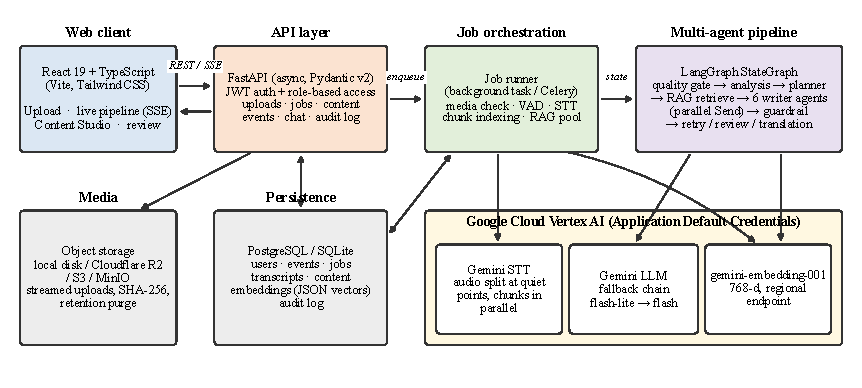
\includegraphics[width=\textwidth]{fig_architecture}
  \caption{EventAI architecture. Arrows show request and data flow; all model calls use
  Vertex AI with Application Default Credentials.}
  \label{fig:arch}
\end{figure*}

\subsection{Ingestion and speech-to-text}
An organiser uploads audio, video or a text transcript after confirming that participants
consented to processing. The job runner validates the file (extension whitelist, size and
duration limits, optional ClamAV scan), measures duration, sample rate and silence ratio, and
applies a voice-activity pre-check that rejects recordings with no detectable speech.
Transcription uses Gemini on Vertex AI. Because Vertex accepts at most about 20\,MB of inline
audio per request, the recording is resampled to 16\,kHz mono and split into windows of
300\,s; each window end is moved to the quietest 250\,ms frame within the preceding 10\,s so
that boundaries fall between words. Chunks are transcribed concurrently (four at a time)
and concatenated. If the engine fails, the runner tries every other configured engine
(Gemini API, VideoDB) in turn, skipping engines whose credentials were rejected at start-up.

\subsection{Multi-agent pipeline}
The pipeline is a LangGraph \texttt{StateGraph} (Fig.~\ref{fig:pipeline}). A quality gate
routes low-confidence transcripts to \texttt{needs\_reupload}. An \emph{analysis} node
extracts topics, highlights, speaker characteristics, tone and an editorial brief (angle,
key messages, audience, verbatim quotes) in one structured JSON call; a \emph{planner} node
reuses this brief. After selective RAG (Section~\ref{sec:rag}), the LangGraph \texttt{Send}
API fans out to the six requested writer agents in parallel: executive summary, blog
article, LinkedIn post, newsletter, Instagram caption and event flyer. Each agent is defined
by a Markdown \emph{skill} file (persona, structure, do/don't rules, an example) plus the
author's profile (name, organisation, tone, sign-off). Writers see the first 12{,}000
characters of the transcript, the brief and the retrieved excerpts, and must return JSON.

\begin{figure*}[t]
  \centering
  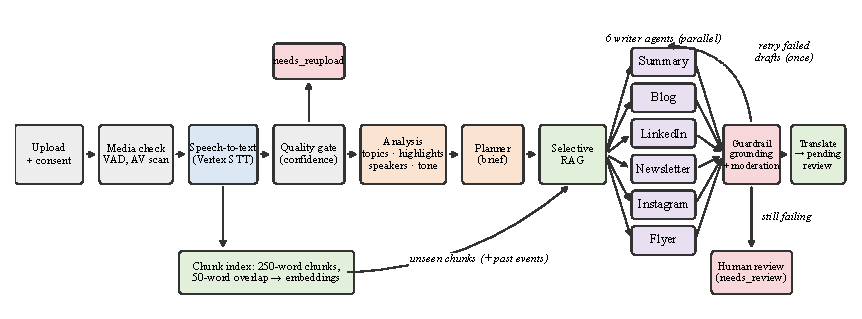
\includegraphics[width=\textwidth]{fig_pipeline}
  \caption{LangGraph pipeline. Only drafts that fail the guardrail are regenerated, once;
  drafts still failing are routed to human review, the rest are translated.}
  \label{fig:pipeline}
\end{figure*}

\subsection{Guardrail and human review}
A single batched LLM call checks all drafts at once for \emph{grounding} (claims not
supported by the transcript) and \emph{moderation}. The guardrail receives the full
transcript and the author profile, so that user-supplied sign-offs are not flagged as
invented. Drafts that fail are regenerated once---only the failing types, skipping the
planner---and drafts that still fail are routed to human review; otherwise the job proceeds
to translation, in which each target language is one batched call for all drafts. Every
draft then waits for approval in the Content Studio, where it can be edited, approved,
copied or exported; nothing is marked ready to publish automatically.

\subsection{Selective retrieval-augmented generation}\label{sec:rag}
Transcripts are split into overlapping 250-word chunks (50-word overlap) and embedded with
\texttt{gemini-embedding-001} (768 dimensions); vectors are stored in a JSON column, so no
database extension is needed. Retrieval is \emph{selective}: it runs only when the
transcript exceeds what the writers see directly ($>$2{,}000 words) or when the organiser
enables organisation memory. The candidate pool excludes chunks already inside the writers'
12{,}000-character excerpt and, with organisation memory, adds chunks from the organiser's
earlier events. A \texttt{rag\_retrieve} graph node builds the query from the editorial
brief (angle, key messages, topics and highlights) and passes the top $k{=}6$ chunks, by
cosine similarity, to every writer, labelled as later parts of this session or as earlier
events that must not be presented as said in this session. If the embedding service is
unavailable, a hashed bag-of-words representation is used instead.

\subsection{Resilience}
Every model call has a timeout (60\,s) and an immediate retry for transient errors. The
Vertex provider always starts with the configured model and walks a fallback chain
(\texttt{gemini-3.1-flash-lite}, then \texttt{gemini-3.6-flash}) when a model returns an
error, a permanent ``not found'' or an empty response. Each model has its own circuit
breaker: after three consecutive failed calls the model is skipped for 60\,s and then tried
again; a model that answered ``not found'' is skipped for the rest of the process. Every
model reply is coerced to a JSON object. If every model fails, an offline template generator
keeps the job running, but the job is flagged as degraded and routed to human review.
Provider credentials are checked at start-up, and speech-to-text falls back through every
configured engine whose credentials were accepted. This is the version after the fixes of
Section~\ref{sec:discussion}; the differences to the version used in most live runs are
listed there.

\subsection{Implementation}
The backend is Python 3.11 (FastAPI 0.115, LangGraph 0.3.31, SQLAlchemy 2.0, google-genai);
the frontend is React~19, TypeScript and Vite with Tailwind CSS. The system is configured by
environment variables (provider, models, RAG threshold, $k$, embedding region) and ships with
Docker Compose files.

\section{Evaluation Methodology}\label{sec:method}
We follow a hybrid, cost-aware protocol: automated local tests with mocked providers, a pilot
on two talks, live end-to-end runs on the whole dataset, cached-stage experiments that reuse
stored transcripts, and mock-based fault injection. Every result is labelled as live,
cached-stage, mock, dataset-based or automatic-judge.

\subsection{Dataset}
We use the long-form release of TED-LIUM~3~\cite{hernandez2018tedlium} (CC BY-NC-ND~3.0, used
for non-commercial academic evaluation only): 19 complete TED talks whose official segments
are concatenated per talk, each with its human reference transcript. One 5.5\,s item is
excluded as it is not a talk, leaving \DatasetTalks{} talks (\DatasetHours{}\,h; \DatasetMinMin--\DatasetMaxMin{}\,min,
median \DatasetMedMin{}\,min) of which \DatasetLong{} exceed 2{,}000 words and therefore
trigger selective RAG. TED talks are recorded conference presentations, i.e.\ the target
domain of EventAI.

\subsection{Execution environment}
All live runs use the unmodified backend, driven in-process through its HTTP routes
(\texttt{POST /uploads}, \texttt{POST /jobs/\{id\}/regenerate}) by a harness that only wraps
functions to record wall-clock timings and the token counts returned by the SDK. Each
worker uses its own SQLite database. Configuration: Vertex AI (\texttt{global} endpoint for
generation, \texttt{asia-south1} for embeddings), \texttt{gemini-3.1-flash-lite} for
transcription, analysis, writing, guardrail and translation, \texttt{gemini-embedding-001}
for RAG, six formats in English plus Hindi translation, and a fixed neutral author profile.
The provider's in-process state (model memory, circuit breakers) is reset before each run so
that every run starts on the configured model. The live runs used the version before the fixes
of Section~\ref{sec:discussion}, except the seven runs of \emph{Elizabeth Gilbert}, which
failed with that version and were repeated after the response-shape fix. The fixes change
behaviour only when calls fail or replies are malformed; in the other runs the only such
events were the failed calls during network outages (Section~\ref{sec:reliability}). Two jobs ran concurrently on a Windows~11 laptop over a home broadband
connection. Runs affected by machine-wide network outages (a single call stalled for
$>$600\,s, or connections refused) are excluded from latency statistics, reported in
Section~\ref{sec:results}, and re-run where needed.

\subsection{Experiments and metrics}
\textbf{E1 Software tests.} The project's pytest suite (offline fake providers) with line
coverage.

\textbf{E2 Speech recognition.} Word and character error rate (WER/CER) against the human
references after the Whisper English normaliser~\cite{radford2023whisper}, as in the ESB
protocol~\cite{gandhi2022esb}, with \texttt{<unk>} tokens removed from references; we report
corpus WER ($\sum (S{+}D{+}I)/\sum N$), per-talk WER and the real-time factor (RTF,
processing time / audio duration). A cached-stage experiment compares three Gemini models
and three chunk lengths using the app's own \texttt{transcribe\_file} function.

\textbf{E3 Latency and tokens.} Per-stage wall time and token usage of the \DatasetTalks{}
live end-to-end runs (upload to finished drafts).

\textbf{E4 Retrieval.} Human reference transcripts of the \DatasetLong{} long talks are
chunked exactly as in the app. For each talk the judge model writes ten factual questions,
each with a verbatim supporting quote; a question is kept only if the quote occurs verbatim
in the reference, and the relevant chunks are those containing it, so relevance is
determined mechanically. We compare \texttt{gemini-embedding-001}, the hashed bag-of-words
vectors used by the previous version of EventAI, and Okapi BM25~\cite{robertson2009bm25}
with Recall@$k$, MRR and nDCG@6~\cite{jarvelin2002ndcg}, both within a talk (the default)
and across all talks (organisation-memory setting).

\textbf{E5 RAG ablation.} For each long talk, the stored transcript is regenerated three
times with RAG on and three times with RAG off, alternating conditions. The judge lists ten
key points per talk from the human reference with verbatim quotes; a point is \emph{late} if
its quote lies beyond the share of the talk the writers see directly. Coverage of early and
late points per draft is averaged per talk and condition and compared with the paired
Wilcoxon signed-rank test~\cite{wilcoxon1945} over talks.

\textbf{E6 Content quality.} Each English draft of the end-to-end runs is scored 1--5 on
factual consistency, relevance, completeness, readability and instruction adherence, with
a list of unsupported claims, by \texttt{gemini-3.7-flash} at temperature 0 against the
human reference transcript (G-Eval-style LLM-as-a-judge~\cite{liu2023geval,zheng2023judging}),
blind to the condition. A second judge (\texttt{gemini-3.6-flash}) re-scores the end-to-end
runs; we report exact agreement, agreement within one point and quadratic weighted
$\kappa$~\cite{cohen1968kappa}. Deterministic format checks (word limits, hashtag counts,
banned phrases, invented dates) complement the judge.

\textbf{E7 Reliability.} \emph{Live}: API errors, empty responses, model fallbacks, guardrail
retries and job outcomes over all live runs. \emph{Mock}: nine fault scenarios $\times$ 20
trials injected into the production Vertex provider and retry code through a fake client,
keeping the real back-off sleeps; plus probes of the circuit breaker and of a sustained rate
limit on the primary model. The mock experiment was run before and after the fixes.

\textbf{E8 Usability walkthrough.} The web client is driven with Playwright (Microsoft Edge)
through registration, upload, the live pipeline view, the Content Studio and review, on a
TED talk, to document the user-facing workflow (Fig.~\ref{fig:ui}).

\section{Results}\label{sec:results}
All numbers below are generated by the released analysis script from saved raw results.

\subsection{E1: Software tests}
\begin{table}[t]
\centering
\caption{Automated test suite (pytest, offline fake providers).}
\label{tab:tests}
\footnotesize
\setlength{\tabcolsep}{3.5pt}
\begin{tabular}{lr}
\toprule
Item & Value \\
\midrule
Test cases (files) & 80 (14) \\
Passed / failed / errors & 80 / 0 / 0 \\
Line coverage (app) & 65.9\% of 3644 statements \\
Coverage: core / graphs / services & 93.8 / 66.8 / 54.1\% \\
Coverage: providers / api & 62.7 / 59.5\% \\
Wall time & 41.9 s \\
\bottomrule
\end{tabular}
\end{table}

The suite (Table~\ref{tab:tests}) passes completely; it includes ten regression tests added
for the fixes described in Section~\ref{sec:discussion} (circuit breaker, model selection,
response shape, degraded-output flag, credential check and speech-to-text fallback chain).
Coverage is lowest for the speech-to-text providers and the job runner's media path, which
the offline suite deliberately does not call; those paths are exercised by the live
experiments below.

\subsection{E2: Speech recognition}
\begin{table*}[t]
\centering
\caption{Speech recognition on TED-LIUM~3 talks (WER/CER in \%, Whisper normaliser). The first row is the production configuration inside the live pipeline; the others are cached-stage runs of the same \texttt{transcribe\_file} function, four configurations processed concurrently.}
\label{tab:asr}
\footnotesize
\setlength{\tabcolsep}{3.5pt}
\begin{tabular}{lrrrrrrrrr}
\toprule
Model & Chunk (s) & Talks & Corpus WER & Median & Max & CER & S/D/I & RTF & STT (s) \\
\midrule
3.1-flash-lite (pipeline) & 300 & 18 & 2.19 & 2.22 & 5.45 & 1.15 & 464/224/284 & 0.048 & 43.2 \\
3.1-flash-lite & 120 & 18 & 2.19 & 2.17 & 5.03 & 1.17 & 460/229/279 & 0.037 & 25.5 \\
3.1-flash-lite & 600 & 18 & 2.23 & 2.34 & 5.38 & 1.17 & 463/227/297 & 0.030 & 24.1 \\
3.6-flash & 300 & 18 & 2.10 & 1.89 & 5.10 & 1.09 & 413/242/276 & 0.041 & 30.8 \\
3.7-flash & 300 & 18 & 1.98 & 1.87 & 4.54 & 1.06 & 380/210/285 & 0.106 & 90.7 \\
\bottomrule
\end{tabular}
\end{table*}

\begin{figure}[t]
  \centering
  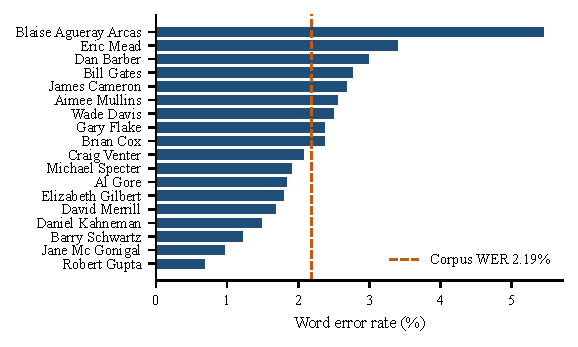
\includegraphics[width=\columnwidth]{fig_wer_per_talk}
  \caption{Per-talk WER of the production configuration (live pipeline, 18 talks).}
  \label{fig:wer}
\end{figure}
In the live pipeline, \texttt{gemini-3.1-flash-lite} with 300\,s quiet-point chunks reaches a
corpus WER of 2.19\% over 44{,}283 reference words (Table~\ref{tab:asr}); per-talk WER ranges
from 0.68\% to 5.45\% (Fig.~\ref{fig:wer}) and the median real-time factor is 0.048; the
longest (25-minute) talk was transcribed in 54\,s. Chunk length barely affects accuracy
(2.19\%, 2.19\% and 2.23\% for 120, 300 and 600\,s windows), which indicates that the
quiet-point splitting does not cut words. The larger \texttt{gemini-3.6-flash} lowers corpus WER
only slightly, to 2.10\%. The newest \texttt{gemini-3.7-flash} is the most accurate (1.98\%)
but more than twice as slow (median RTF 0.106, 90.7\,s per talk), and 10 of its 28
transcription attempts failed---in three talks chunks exceeded the 240\,s per-chunk timeout, the
others coincided with network outages---and were repeated until all 18 talks succeeded. The production choice of \texttt{flash-lite} therefore
trades 0.2 WER points for less than half the transcription time (Fig.~\ref{fig:asrmodels}).
\begin{figure}[t]
  \centering
  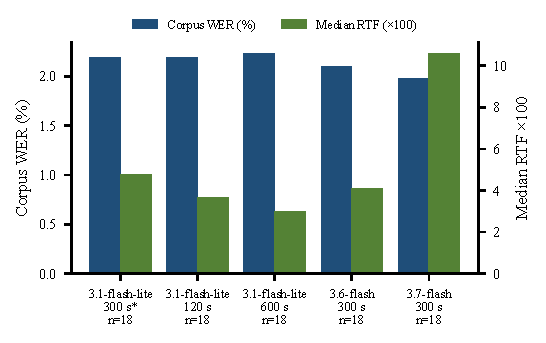
\includegraphics[width=\columnwidth]{fig_asr_models}
  \caption{Corpus WER and median real-time factor by model and chunk length (* = live pipeline).}
  \label{fig:asrmodels}
\end{figure}
Across talks, WER is not related to the judged quality of the drafts (Spearman $\rho=-0.09$,
$n=18$), consistent with the low error rate. Substitutions are the most
frequent error type (464, against 224 deletions and 284 insertions). Transcription consumed 1{,}500--2{,}000 input tokens
per minute of audio, depending on the chunk length.

\subsection{E3: Latency and token usage}
\begin{table}[t]
\centering
\caption{Per-stage latency of the live end-to-end runs (seconds; completed jobs, upload to finished drafts incl.\ Hindi translation).}
\label{tab:latency}
\footnotesize
\setlength{\tabcolsep}{3.5pt}
\begin{tabular}{lrrrr}
\toprule
Stage & $n$ & Median & IQR & Range \\
\midrule
Media check & 18 & 12.30 & 4.55--14.72 & 3.00--155.35 \\
Speech-to-text & 18 & 43.24 & 21.13--51.99 & 8.45--135.53 \\
RAG indexing & 18 & 1.74 & 1.09--2.99 & 0.60--10.09 \\
Analysis & 18 & 3.14 & 2.92--3.27 & 2.64--3.70 \\
RAG retrieval & 18 & 0.57 & 0.00--0.73 & 0.00--0.99 \\
Generation (6 agents) & 18 & 5.41 & 5.02--5.78 & 4.25--10.13 \\
Guardrail (+retry) & 18 & 2.04 & 1.73--2.37 & 1.49--8.40 \\
Translation (hi) & 18 & 12.49 & 11.55--12.92 & 11.10--13.75 \\
\midrule
Total (upload to drafts) & 18 & 90.20 & 56.40--98.20 & 32.90--226.30 \\
\bottomrule
\end{tabular}
\end{table}

\begin{figure}[t]
  \centering
  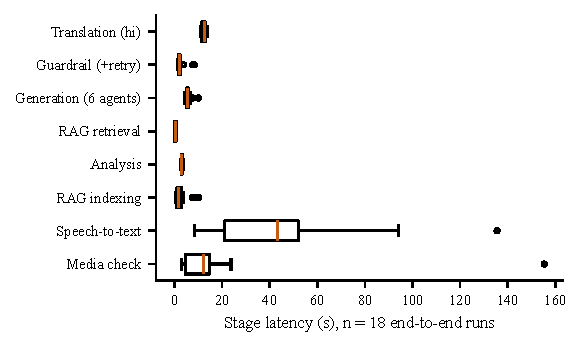
\includegraphics[width=\columnwidth]{fig_latency_stages}
  \caption{Stage latency distribution of the live end-to-end runs.}
  \label{fig:latency}
\end{figure}
\begin{figure}[t]
  \centering
  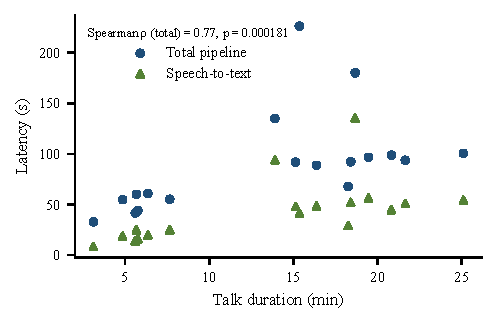
\includegraphics[width=\columnwidth]{fig_latency_vs_duration}
  \caption{Talk duration versus total and speech-to-text latency.}
  \label{fig:latdur}
\end{figure}
A completed job---transcription, analysis, six drafts, guardrail and a Hindi translation of
all drafts---took a median of 90.2\,s (IQR 56.4--98.2\,s) for talks with a median length of
15.2\,min, i.e.\ a median end-to-end real-time factor of 0.12 (Table~\ref{tab:latency},
Fig.~\ref{fig:latency}). Speech-to-text dominates (median 43.2\,s), followed by the local media
check (local silence analysis, median 12.3\,s, with one outlier of 155\,s) and translation
(12.5\,s). Thanks to the parallel fan-out, writing all six drafts takes
only 5.4\,s (median); analysis (3.1\,s), the guardrail (2.0\,s) and RAG retrieval (0.6\,s) are
minor. Total latency grows with talk length (Spearman $\rho=0.77$, $p=1.8\times10^{-4}$,
$n=18$; Fig.~\ref{fig:latdur}). A job made on average 12.8 LLM calls and used 64.5\,k input and
12.0\,k output tokens, of which the six writers account for 28.8\,k input tokens and
transcription for 21.8\,k audio tokens (Fig.~\ref{fig:tokens}).

\begin{figure}[t]
  \centering
  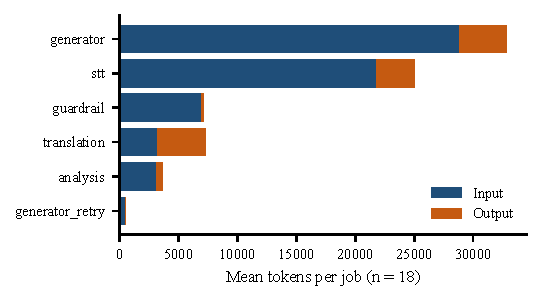
\includegraphics[width=\columnwidth]{fig_tokens_stage}
  \caption{Mean tokens per job by stage (live end-to-end runs).}
  \label{fig:tokens}
\end{figure}

\subsection{E4: Retrieval quality}
\begin{table*}[t]
\centering
\caption{Retrieval on 109 labelled questions over 181 chunks of 11 long talks.}
\label{tab:retrieval}
\footnotesize
\setlength{\tabcolsep}{3.5pt}
\begin{tabular}{llrrrrr}
\toprule
Pool & Retriever & R@1 & R@3 & R@6 & MRR & nDCG@6 \\
\midrule
within-talk & gemini-embedding-001 & 0.76 & 0.98 & 1.00 & 0.87 & 0.90 \\
within-talk & hashed bag-of-words (prev.) & 0.23 & 0.49 & 0.61 & 0.41 & 0.41 \\
within-talk & BM25 & 0.57 & 0.89 & 0.93 & 0.73 & 0.77 \\
\midrule
cross-talk & gemini-embedding-001 & 0.74 & 0.96 & 0.98 & 0.85 & 0.88 \\
cross-talk & hashed bag-of-words (prev.) & 0.06 & 0.14 & 0.21 & 0.13 & 0.12 \\
cross-talk & BM25 & 0.54 & 0.80 & 0.84 & 0.68 & 0.71 \\
\bottomrule
\end{tabular}
\end{table*}

\begin{figure}[t]
  \centering
  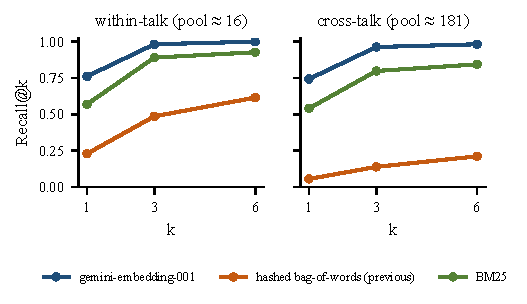
\includegraphics[width=\columnwidth]{fig_retrieval}
  \caption{Recall@$k$ of the three retrievers within a talk and across all talks.}
  \label{fig:retrieval}
\end{figure}
Of 110 generated questions, 109 had a quote found verbatim in the reference and were kept. With
\texttt{gemini-embedding-001}, the relevant chunk is ranked first for 76\% of the questions and
is always within the top six that EventAI passes to the writers (Recall@6 = 1.00, MRR 0.87;
Table~\ref{tab:retrieval}, Fig.~\ref{fig:retrieval}). BM25 is a strong lexical baseline
(MRR 0.73), while the hashed bag-of-words vectors of the previous EventAI version reach only
MRR 0.41. The gap widens in the organisation-memory setting with 181 candidate chunks from
eleven talks: the embedding retriever keeps Recall@6 at 0.98, whereas hashed vectors collapse to
0.21, i.e.\ they could not have supported cross-event memory.

\subsection{E5: Effect of selective RAG}
\begin{table}[t]
\centering
\caption{RAG ablation: same stored transcript, 3 runs per condition, averaged per talk ($n=11$ long talks); two-sided Wilcoxon signed-rank test. Coverage from the automatic judge.}
\label{tab:rag}
\footnotesize
\setlength{\tabcolsep}{2.2pt}
\begin{tabular}{lrrrrr}
\toprule
Metric & RAG off & RAG on & $\Delta$ & $+$/$-$ & $p$ \\
\midrule
Late coverage, all formats (\%) & 46.8 & 68.4 & +21.6 & 10/0 & 0.0020 \\
Early coverage, all formats (\%) & 70.1 & 58.5 & -11.6 & 1/10 & 0.0029 \\
Late coverage, long formats (\%) & 50.8 & 74.7 & +23.9 & 9/0 & 0.0039 \\
All key points, all formats (\%) & 59.8 & 59.1 & -0.7 & 5/5 & 0.7148 \\
\midrule
Factual cons. & 4.96 & 4.99 & +0.03 & 4/1 & 0.1875 \\
Relevance & 5.00 & 4.97 & -0.03 & 0/2 & 0.5000 \\
Completeness & 4.20 & 4.28 & +0.08 & 7/3 & 0.3223 \\
Readability & 5.00 & 4.96 & -0.03 & 1/2 & 0.5000 \\
Instr. adherence & 4.67 & 4.69 & +0.02 & 4/6 & 0.7090 \\
Unsupported claims per draft & 0.04 & 0.01 & -0.04 & 1/5 & 0.1250 \\
\bottomrule
\end{tabular}
\\[2pt]\parbox{\linewidth}{\scriptsize $+$/$-$: talks whose per-talk mean rose/fell with RAG.}
\end{table}

\begin{figure}[t]
  \centering
  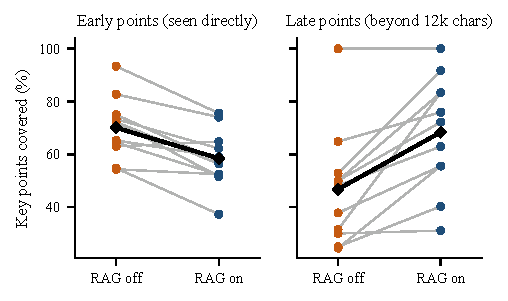
\includegraphics[width=\columnwidth]{fig_rag_ablation}
  \caption{Key-point coverage per talk without and with RAG (grey lines: talks; black: mean).}
  \label{fig:rag}
\end{figure}
On the eleven long talks, RAG raised coverage of key points that lie beyond the writers'
12{,}000-character excerpt from 46.8\% to 68.4\% (+21.6 points; 10 of 11 talks improved, none
worse; $p=0.0020$), and from 50.8\% to 74.7\% for the long formats (Table~\ref{tab:rag},
Fig.~\ref{fig:rag}). Coverage of early points fell from 70.1\% to 58.5\% ($p=0.0029$), and
total coverage was unchanged (59.8\% vs.\ 59.1\%, $p=0.71$): with a fixed output length, RAG
\emph{redistributes} the drafts' attention over the whole talk rather than adding content.
Rubric scores, including factual consistency, did not change significantly, and unsupported
claims stayed rare in both conditions (0.01 vs.\ 0.04 per draft). The \emph{Elizabeth Gilbert}
runs were made after the response-shape fix (Section~\ref{sec:discussion}); without them the
result is the same in direction and significance (late coverage 48.4\% to 72.1\%,
$p=0.0039$, $n=10$). For organisers this means
that, with RAG, posts about long talks no longer ignore their second half.

\subsection{E6: Content quality}
\begin{table*}[t]
\centering
\caption{Automatic-judge quality scores (1--5) of the English drafts of the live end-to-end runs, judged against the human reference transcript.}
\label{tab:quality}
\footnotesize
\setlength{\tabcolsep}{3.5pt}
\begin{tabular}{lrrrrrrr}
\toprule
Format & $n$ & Fact. & Rel. & Compl. & Read. & Instr. & Unsup. \\
\midrule
Summary & 18 & 4.94 & 5.00 & 4.72 & 5.00 & 5.00 & 0.06 \\
Blog & 18 & 5.00 & 5.00 & 4.83 & 5.00 & 4.50 & 0.00 \\
Linkedin & 18 & 5.00 & 5.00 & 4.33 & 5.00 & 4.33 & 0.00 \\
Newsletter & 18 & 4.94 & 5.00 & 4.44 & 5.00 & 4.67 & 0.06 \\
Instagram & 18 & 4.94 & 5.00 & 4.06 & 5.00 & 4.94 & 0.06 \\
Flyer & 18 & 4.94 & 5.00 & 3.72 & 5.00 & 4.44 & 0.06 \\
\midrule
All & 108 & 4.96 & 5.00 & 4.35 & 5.00 & 4.65 & -- \\
\bottomrule
\end{tabular}
\end{table*}

\begin{figure}[t]
  \centering
  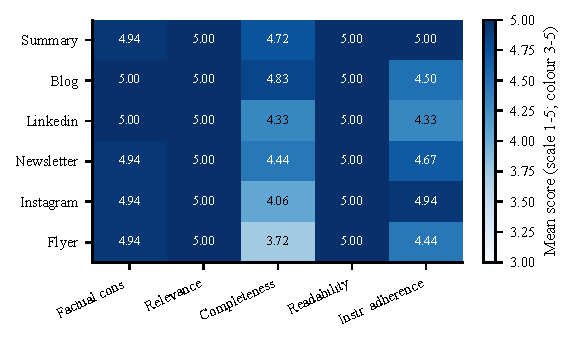
\includegraphics[width=\columnwidth]{fig_quality_heatmap}
  \caption{Mean judge score per format and dimension (colour scale 3--5).}
  \label{fig:quality}
\end{figure}
\begin{table}[t]
\centering
\caption{Deterministic format checks on the end-to-end drafts.}
\label{tab:format}
\footnotesize
\setlength{\tabcolsep}{3.5pt}
\begin{tabular}{lr}
\toprule
Check & Pass \\
\midrule
linkedin 3-5 hashtags & 12/18 \\
linkedin no banned phrases & 18/18 \\
instagram 10-15 hashtags & 18/18 \\
summary <= 400 words & 18/18 \\
flyer no invented date (TBA or none) & 18/18 \\
\bottomrule
\end{tabular}
\end{table}

\begin{table}[t]
\centering
\caption{Agreement between the primary judge (J1, gemini-3.7-flash) and a second judge (J2, gemini-3.6-flash) on the same drafts.}
\label{tab:judge}
\footnotesize
\setlength{\tabcolsep}{3.5pt}
\begin{tabular}{lrrrrrr}
\toprule
Dimension & $n$ & Exact \% & $\pm$1 \% & QWK & J1 & J2 \\
\midrule
Factual cons. & 108 & 90.7 & 100.0 & 0.25 & 4.96 & 4.91 \\
Relevance & 108 & 100.0 & 100.0 & -- & 5.00 & 5.00 \\
Completeness & 108 & 73.1 & 100.0 & 0.62 & 4.35 & 4.32 \\
Readability & 108 & 99.1 & 100.0 & 0.00 & 5.00 & 4.99 \\
Instr. adherence & 108 & 89.8 & 100.0 & 0.88 & 4.65 & 4.69 \\
\bottomrule
\end{tabular}
\end{table}

Judged against the human transcript, the 108 English drafts of the 18 end-to-end
runs score 4.96 for factual consistency with 0--0.06 unsupported claims per draft, 5.00 for
relevance and readability, 4.65 for instruction adherence and 4.35 for completeness
(Table~\ref{tab:quality}, Fig.~\ref{fig:quality}). Completeness is lowest for the short
formats---Instagram (4.06) and especially the flyer (3.72)---which is expected from their
length limits. The deterministic checks (Table~\ref{tab:format}) confirm summary length,
Instagram hashtag counts, absence of banned LinkedIn clich\'es and absence of invented event
dates in all drafts, but only 12 of 18 LinkedIn posts respect the 3--5 hashtag rule. The two
judges agree within one point on every item and exactly on 73.1--100\% of items per dimension
(Table~\ref{tab:judge}); weighted $\kappa$ is 0.62 for completeness and 0.88 for instruction
adherence, and is low or undefined for relevance, readability and factual consistency only
because almost all scores are 5 (the well-known $\kappa$ paradox at a ceiling). The high scores
should therefore be read as ``no defects detected by two LLM judges'' rather than as human
ratings.

\subsection{E7: Reliability}\label{sec:reliability}
\begin{table*}[t]
\centering
\caption{Mock-based fault injection into the production Vertex provider (20 trials per scenario). ``Next call'' is the first model tried by the next call in the same process; ``Flagged'' counts trials whose fallback output was marked as degraded.}
\label{tab:faults}
\footnotesize
\setlength{\tabcolsep}{3.5pt}
\begin{tabular}{llrrlr}
\toprule
Scenario & Outcome (of 20) & Calls & Lat. (s) & Next call & Flagged \\
\midrule
S0 no fault & primary model 20 & 1.0 & 0.00 & 3.1-flash-lite & 0 \\
S1 transient 429 (once) & primary model 20 & 2.0 & 0.00 & 3.1-flash-lite & 0 \\
S2 timeout (once) & primary model 20 & 2.0 & 0.00 & 3.1-flash-lite & 0 \\
S3 persistent 429 on primary & fallback model 20 & 4.0 & 1.01 & 3.1-flash-lite & 0 \\
S4 model 404 not found & fallback model 20 & 2.0 & 0.00 & 3.6-flash & 0 \\
S5 empty response & fallback model 20 & 2.0 & 0.00 & 3.1-flash-lite & 0 \\
S6 JSON in markdown fence & primary model 20 & 1.0 & 0.00 & 3.1-flash-lite & 0 \\
S7 prose, no JSON & unparsed (raw text) 20 & 1.0 & 0.00 & 3.1-flash-lite & 0 \\
S8 all models 500 & offline template 20 & 6.0 & 2.02 & 3.1-flash-lite & 20 \\
\bottomrule
\end{tabular}
\\[2pt]\parbox{\linewidth}{\scriptsize Circuit-breaker probe: 8 consecutive failing calls (fail\_max = 5) reached the upstream 5 times; 3 were short-circuited. Sustained 429 on the primary over 8 calls: the primary was tried by 3 calls, then skipped by its model breaker (fail\_max = 3, 60\,s window).}
\end{table*}

\begin{figure}[t]
  \centering
  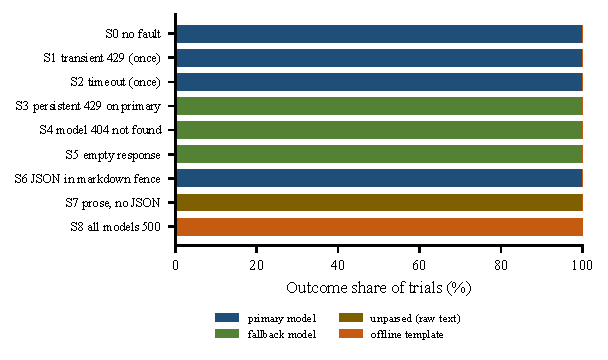
\includegraphics[width=\columnwidth]{fig_fault_injection}
  \caption{Outcomes of mock fault injection (20 trials per scenario).}
  \label{fig:faults}
\end{figure}
\emph{Live.} Across 93 live pipeline runs (84 planned, two repeated after outages and the seven
\emph{Elizabeth Gilbert} runs repeated after the response-shape fix) the backend made 946 model
and embedding calls; 22 failed (2.3\%): 2 rate-limit (429) responses, 7 timeouts and 13 network
errors during host outages. No empty responses and no model fallbacks occurred. The guardrail
triggered a targeted regeneration in 8 runs; after it, 2 of 510 final English drafts (both
newsletters) remained flagged and their jobs were routed to human review. 83 jobs reached
\texttt{pending\_review}, 2 \texttt{needs\_review} and 8 failed: the 7 \emph{Elizabeth Gilbert}
runs before the response-shape fix (all 7 repeated runs after it completed) and 1 from a
network outage combined with an invalid fallback STT credential.

\emph{Mock.} Transient 429s, timeouts, unknown models, empty responses and fenced JSON are all
recovered with usable output (Table~\ref{tab:faults}, Fig.~\ref{fig:faults}); persistent rate
limiting costs about 1\,s before the fallback model answers. Prose without any JSON is still
passed on unparsed. Before the fixes, the next call after an empty response or a persistent
429 stayed on the fallback model (sticky fallback), the circuit breaker short-circuited none of
8 consecutive failing calls, and offline template text was returned without any flag. After
them, the next call returns to the primary model, the breaker rejects 3 of the 8 calls, a
persistently rate-limited primary is skipped from the fourth call on, so later calls no longer
pay the 1\,s, and all 20 trials in which every model failed are flagged as degraded.

\subsection{E8: User-facing workflow}
\begin{figure*}[t]
  \centering
  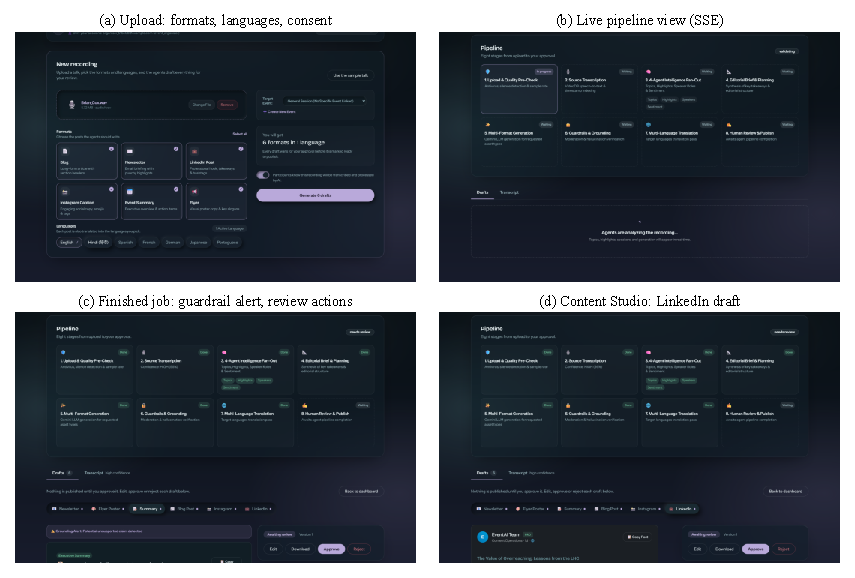
\includegraphics[width=\textwidth]{fig_ui}
  \caption{EventAI web client operated by Playwright on a TED talk: (a) upload with format,
  language and consent selection; (b) live pipeline view; (c) finished job, where the guardrail
  flagged one draft and the job awaits review; (d) a LinkedIn draft in the Content Studio.}
  \label{fig:ui}
\end{figure*}
Fig.~\ref{fig:ui} shows the workflow captured by Playwright on the 3-minute \emph{Brian Cox}
talk: an organiser selects formats, languages and confirms consent, follows the pipeline
stages live and reviews, edits, approves or rejects each draft. In this run the guardrail
flagged the summary and the job correctly stopped at \texttt{needs\_review}. The walkthrough
also exposed a stale label in the client (the transcription stage still named VideoDB, which
the deployment no longer uses); it was corrected after the walkthrough.

\section{Discussion}\label{sec:discussion}
\subsection{Defects exposed by the evaluation}
Running the real system on real talks surfaced problems that the offline test suite, which
uses fake providers, could not reveal. We report them because they are the most practically
useful outcome for practitioners building similar pipelines.

\textbf{Guardrail scope (fixed before the final runs).} The guardrail originally saw only
the first 12{,}000 transcript characters and not the author profile. In the pilot, all six
drafts of a talk were flagged: user-supplied sign-offs were reported as ``invented'', and
correct facts from late in the talk (supplied to the writers by RAG) would have been
penalised. The guardrail now receives the whole transcript and the profile.

\textbf{Few-shot template leakage (fixed).} The flyer and summary skill files contained
example outputs with a concrete date (``October~24, 2026'') and a venue, and the flyer rules
demanded a date. With no event metadata available, writers copied the example date into
drafts; the guardrail caught it, but only after a regeneration round-trip. A shared rule
forbidding copying of example details and requiring ``TBA'' for unknown logistics removed
the behaviour (Table~\ref{tab:format}).

\textbf{Sticky model fallback (fixed after the evaluation).} The Vertex provider remembered the
last working model for the whole process. In the pilot, a single empty response from
\texttt{gemini-3.1-flash-lite} switched every subsequent call of the process to the larger
\texttt{gemini-3.6-flash}, silently changing quality, latency and cost. The provider now always
starts with the configured model and skips a model only while its own circuit breaker is open
(three consecutive failures, 60\,s). In the repeated fault injection the next call returns to
\texttt{gemini-3.1-flash-lite} after an empty response and after a persistent 429
(Table~\ref{tab:faults}).

\textbf{Inert circuit breaker (fixed after the evaluation).} The circuit breaker recorded
failures but its \texttt{allow()} method never raised, so it never short-circuited a call. It
now rejects calls while open and lets one trial call through after the window (half-open).
The probe now shows 3 of 8 consecutive failing calls short-circuited (0 before), and the
per-model breakers mean that a rate-limited primary costs the back-off delay only on the first
three calls (Section~\ref{sec:reliability}).

\textbf{Silent offline fallback (fixed after the evaluation).} When every model failed, the
provider returned offline template text and the job looked like a normal result. Every step
that falls back (offline template, placeholder draft, missing translation) now marks the job
as degraded; such a job ends in \texttt{needs\_review} with an explanatory message. All 20
fault-injection trials in which every model failed are flagged.

\textbf{Unguarded response shape (fixed after the evaluation).} In
\LiveAnalysisShapeFailures{} live runs---every run of one talk (\emph{Elizabeth Gilbert})---the
analysis model returned a JSON array instead of an object, the analysis node raised
\texttt{'list' object has no attribute 'get'} and the job failed. The failure is deterministic
for that input, so retries did not help. Replies are now coerced to an object (an array of
objects is unwrapped and merged), and the analysis node re-asks once with an explicit
instruction if the expected keys are still missing. With the fix all seven runs of the talk
completed, each with a single analysis call, and the talk is included in the ablation and
quality results.

\textbf{Regional endpoints matter.} Embedding calls on Vertex's \texttt{global} endpoint took
about 12\,s each from our location versus 0.5--0.7\,s on regional endpoints; moving
embeddings to \texttt{asia-south1} removed RAG indexing from the critical path.

\textbf{Network resilience of the host.} Several runs coincided with machine-wide network
outages (DNS failures, SSL errors, stalled connections). Because token refresh in the
Google client is synchronous, a stalled refresh blocks the event loop and the per-call
timeout cannot fire; one call stalled for over 80 minutes before completing. The fallback
STT engine (Gemini API) also failed in these cases because its API key was invalid, and the
runner did not fall back a second level. Credentials of every configured engine are now
checked at start-up, a rejected engine is skipped, and speech-to-text tries every remaining
engine in turn (fixed after the evaluation). Following these stalls we added a 240\,s per-chunk timeout to
the Vertex STT provider; the end-to-end runs used the version without it, the later
cached-stage transcription runs the version with it.

\subsection{Threats to validity}
\emph{Sample size}: \DatasetTalks{} talks and \DatasetLong{} long talks are enough for paired
non-parametric tests and descriptive statistics, not for fine-grained claims; confidence
intervals are wide. \emph{Domain}: TED talks are well-recorded, single-speaker English
talks; noisy multi-speaker event audio would raise WER. \emph{Automatic judging}: quality
scores come from an LLM judge, not human raters; we use a different, larger judge model,
blind conditions, a human reference transcript and a second judge, but judge bias towards
fluent text remains. Key points are model-extracted (with verbatim quotes checked
mechanically). \emph{Retrieval labels} are produced by construction from model-written
questions and may favour paraphrase-friendly queries. \emph{Environment}: latency was
measured on a consumer laptop and home network with two concurrent jobs; absolute numbers
depend on region and load. \emph{Cost}: we report measured tokens; we could not retrieve
official per-token prices for the models used, so monetary cost is not reported.

\section{Conclusion and Future Work}
EventAI shows that a recording-to-publication pipeline built from a multimodal LLM, an explicit
multi-agent graph, a batched guardrail and selective RAG can turn a 15-minute talk into six
review-ready drafts and their translations in about one and a half minutes, at a word error
rate of about 2\% on real talks. The evaluation supports three practical conclusions. First,
parallel writer agents make generation a minor part of latency; transcription and local media
analysis dominate. Second, for long talks a writer that sees only the beginning of the
transcript under-reports the rest; brief-driven retrieval with modern embeddings fixes this
imbalance, but does not by itself make drafts more complete overall. Third, evaluating the
deployed system end to end on real inputs found defects that unit tests with fake providers
could not, so live, instrumented evaluation should be part of building such systems.

The defects found this way---sticky model fallback, an inert circuit breaker, silent offline
fallback, an unguarded response shape and missing credential checks---have been fixed and the
affected experiments re-run. Future work includes: validating every model response against a
full per-step schema rather than only its shape; human evaluation of a sample of drafts to
calibrate the automatic judge; noisy, multi-speaker and Indian-language recordings; and using
event metadata so that flyers can include real logistics instead of ``TBA''.


\section*{Acknowledgment}
The evaluation uses the TED-LIUM~3 corpus (CC BY-NC-ND~3.0) for non-commercial academic
research. Model calls were made on Google Cloud Vertex AI.

\bibliographystyle{IEEEtran}
\bibliography{references}

\end{document}
